\chapter{Machine learning: problems, evidence, and systems}
\label{ch:machine-learning-foundations}

\begin{learningobjectives}
After this chapter, you should be able to:
\begin{itemize}
  \item explain machine learning as the estimation of behavior from data and
  feedback rather than as a catalog of algorithms;
  \item distinguish supervised, unsupervised, self-supervised, generative,
  reinforcement, and causal questions by their information and claim;
  \item identify the representation, hypothesis class, objective, learning
  algorithm, and evaluation distribution in a mathematical learning problem;
  \item explain why inductive bias and out-of-sample evidence are unavoidable;
  and
  \item connect an empirical model to the software and decision system that
  produces, serves, and monitors it.
\end{itemize}
\end{learningobjectives}

\begin{chapterconnection}
Part I built reliable paths from data sources to tested software and operated
services. Part II asks what changes when one component is estimated from data.
The answer is not that ordinary engineering disappears. A learned component
adds a population, a sampling process, an objective, uncertainty, adaptive
selection, and the possibility that future data differ from past data.
\end{chapterconnection}

\section{A short history of a broad idea}

The mathematics now used in machine learning predates the name. Least squares
grew from astronomy and geodesy in the early nineteenth century. Probability,
statistical decision theory, optimization, information theory, control, and
pattern recognition supplied other foundations. By 1950 Alan Turing was
discussing the possibility of a learning machine rather than a machine whose
every response was specified directly.\footnote{A. M. Turing, ``Computing
Machinery and Intelligence,'' \emph{Mind}, 59(236), 1950,
\url{https://doi.org/10.1093/mind/LIX.236.433}.} Arthur Samuel's 1959 checkers
study described a program whose playing behavior improved from experience and
helped establish the term machine learning in computing.\footnote{A. L.
Samuel, ``Some Studies in Machine Learning Using the Game of Checkers,''
\emph{IBM Journal of Research and Development}, 3(3), 1959,
\url{https://doi.org/10.1147/rd.33.0210}.}

This history matters because machine learning is not a single modern invention
and is not synonymous with neural networks. A linear least-squares estimator,
a nearest-neighbor rule, a decision tree, a transformer, and a learned control
policy can all be machine-learning components. Their data, assumptions,
objectives, computation, and evidence differ.

Three historical currents should be kept distinct. Statistics developed rules
for learning about populations from samples. Numerical analysis developed
algorithms for solving the resulting optimization and linear-algebra problems.
Computer science developed representations, programmable procedures, and
systems able to repeat those calculations at scale. Contemporary machine
learning joins all three. It inherits uncertainty from statistics, approximation
and conditioning from numerical analysis, and state, interfaces, testing, and
resource limits from software engineering.

\begin{misconceptionbox}
\textbf{Misconception:} machine learning begins when a sufficiently complicated
model is used. \textbf{Correction:} learning begins when behavior is estimated
from experience under an explicit task and criterion. Complexity alone does
not define learning, and a large model does not remove the need to specify the
problem.
\end{misconceptionbox}

\section{What exactly is learned?}

Let $D$ denote observed experience and let $\mathcal{F}$ be a set of candidate
functions or policies. A learning algorithm is itself a map
\[
\mathcal{A}:D\longmapsto \widehat f_D\in\mathcal{F}.
\]
The output $\widehat f_D$ may predict a number, assign a score, transform an
input into a representation, estimate a distribution, generate an object, or
select an action. The subscript $D$ is essential: another sample, ordering, or
random seed may produce another fitted object.

A complete learning problem contains at least five mathematical choices:

\begin{enumerate}
  \item a \term{representation} $\phi$ that converts available evidence into
  model input $x=\phi(r)$;
  \item a \term{hypothesis class} $\mathcal{F}$ describing candidate behavior;
  \item an \term{objective} that scores candidate behavior on experience;
  \item a \term{learning algorithm} that searches, estimates, or updates; and
  \item an \term{evaluation setting} that defines where performance must
  transfer.
\end{enumerate}

These choices are coupled. Euclidean distance on unscaled chemical
measurements defines a different clustering problem from Euclidean distance
after standardization. Squared loss and absolute loss target different
population summaries. A random row split and a future-time split estimate
performance for different uses. ``The model'' is therefore not just the class
name printed by a library.

\begin{definitionbox}{learning system}
A learning system joins a data-generating process, representation, fitted
component, objective, software interface, decision or scientific consumer,
evaluation design, and feedback path. Its unit of analysis is the claim made by
the complete path, not merely the estimator object.
\end{definitionbox}

\section{Branches are distinguished by information and feedback}

The familiar branches are best treated as problem structures rather than
product labels.

\begin{tabularx}{\textwidth}{@{}p{0.19\textwidth}p{0.28\textwidth}X@{}}
\toprule
Problem structure & Learning information & Typical output and evidence \\
\midrule
Supervised & Inputs paired with observed targets & Numeric prediction, score,
probability, or label; evaluated against held-out targets \\
Unsupervised & Inputs without a supplied target & Clusters, lower-dimensional
coordinates, density, or anomaly score; evaluated by stability, reconstruction,
domain utility, or other task-specific evidence \\
Self-supervised & Targets constructed from the observations & A representation
or predictive model transferred to later tasks \\
Generative & Samples from a distribution, sometimes with conditions & New
samples or likelihood-like scores; evaluated by distributional, task, expert,
and safety evidence \\
Reinforcement & States, actions, and delayed rewards gathered through
interaction & A policy or value function; evaluated by return under an
admissible interaction or off-policy design \\
\bottomrule
\end{tabularx}

These categories overlap. A language model may be pretrained by a
self-supervised objective, adapted with supervised examples, and further
optimized from preference or reward signals. A medical product may use an
unsupervised representation inside a supervised risk model. ``Deep learning''
describes a family of multilayer representations, not a separate source of
feedback.

Causal inference is a neighboring but different claim. Prediction asks about
$Y$ given observed $X$. An intervention asks about an outcome under an action
that may not have occurred. Associational fit alone cannot identify that
counterfactual comparison.

Figure~\ref{fig:learning-landscape} uses four real tables from the course
database to make the distinction visible. The panels are not four competing
algorithms applied to one task. They are four different questions, with
different information and different meanings of success. In the clustering
panel the colors are produced by the algorithm; in the representation panel
the labels are shown only afterward as an audit. That distinction is part of
the experimental design.

\begin{figure}[htbp]
  \centering
  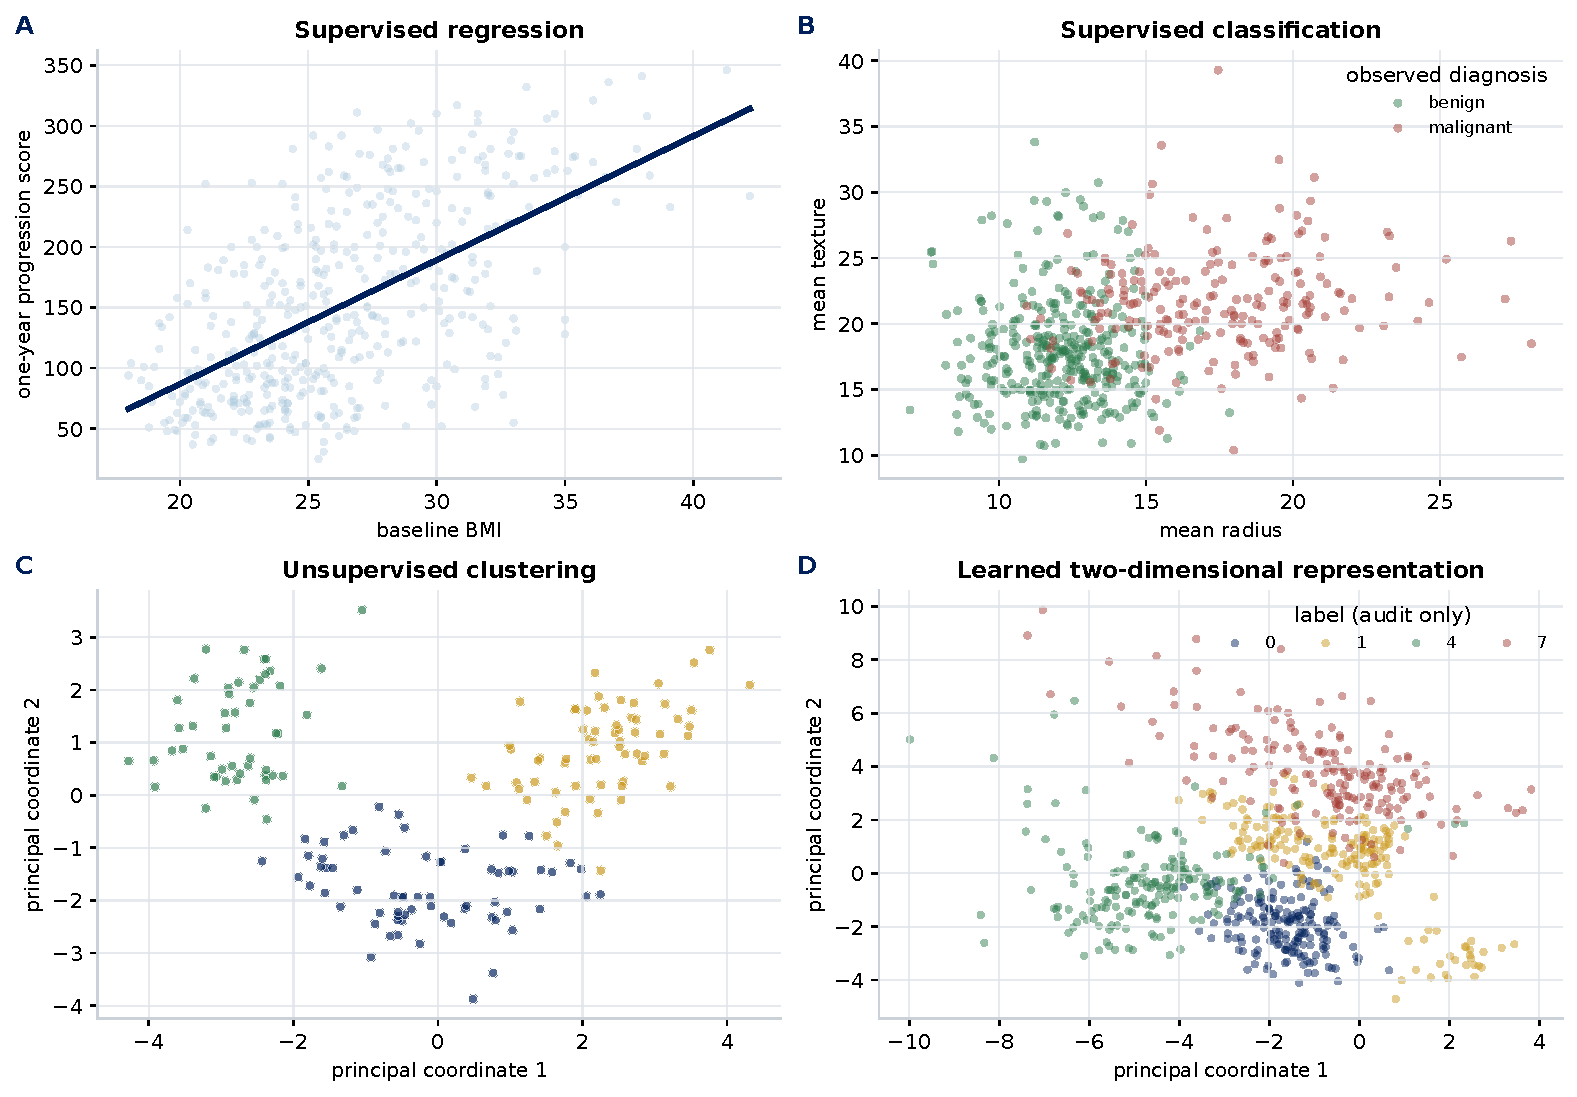
\includegraphics[width=\textwidth]{figures/generated/learning-landscape.pdf}
  \caption{Four learning structures constructed from documented observations
  in the local course database. The plotting program queries SQLite, fits the
  displayed estimators, and writes this vector graphic. Regenerate it with
  \code{uv run python textbook/figures/generate\_part\_ii\_figures.py}.}
  \label{fig:learning-landscape}
\end{figure}

\conceptcheck{A laboratory hides protein labels, learns an embedding from
amino-acid sequences, and then fits a small labeled classifier. Which learning
signals appear in the two stages? Which held-out evidence would be needed to
support the final classification claim?}

\section{Inductive bias is not optional}

Finite observations do not determine behavior everywhere. Infinitely many
functions can interpolate a finite regression sample, and many partitions can
describe an unlabeled cloud. A learner must prefer some continuations over
others. That preference is its \term{inductive bias}.

Bias enters through the representation, model class, loss, regularization,
optimization, initialization, augmentation, stopping rule, and data collection.
A linear model prefers affine relationships. A nearest-neighbor method prefers
local smoothness under a chosen distance. A convolutional architecture encodes
spatial sharing. None is neutral.

\begin{theorem}[Finite interpolation does not determine prediction]
\label{thm:finite-interpolation}
Let $x_1,\ldots,x_n$ be distinct real inputs and suppose a function $f$ fits
the observations, so that $f(x_i)=y_i$ for every $i$. For every real constant
$c$, the function
\[
g_c(x)=f(x)+c\prod_{i=1}^{n}(x-x_i)
\]
fits exactly the same observations. At any $x_*$ different from every $x_i$,
the possible values $g_c(x_*)$ range over all real numbers as $c$ varies.
\end{theorem}

\begin{proof}
At an observed input $x_j$, the product contains the zero factor
$x_j-x_j$, so $g_c(x_j)=f(x_j)=y_j$. At a new input $x_*$, the product
$q=\prod_i(x_*-x_i)$ is nonzero. Hence $g_c(x_*)=f(x_*)+cq$. Because $q\ne0$,
choosing $c=(a-f(x_*))/q$ produces any desired value $a$. The observations
alone therefore cannot select one extrapolation.
\end{proof}

The theorem is elementary, but its force is general: a learner must restrict
the candidate continuations or prefer some over others. Smoothness, sparsity,
a kernel, an architecture, a prior, regularization, and an optimization
trajectory are all possible sources of that preference. Calling the preference
``bias'' does not make it an error; the relevant question is whether it is
defensible for the intended population.

Suppose two functions $f_1$ and $f_2$ agree at every observed $x_i$ but differ
at a future $x_*$. No calculation using only the observed labels can determine
which future value is correct. Generalization becomes possible only through
assumptions connecting observed and future cases. Large datasets can reduce
uncertainty under those assumptions; they do not abolish the assumptions.

\begin{warningbox}
Calling a pipeline ``data driven'' can hide strong human choices. Column
selection, target definition, labeling policy, sampling, missing-value handling,
objective, architecture, and evaluation boundary all shape what the data can
appear to say.
\end{warningbox}

\section{From population risk to empirical evidence}

For supervised prediction with loss $L$, define population risk
\[
R(f)=\mathbb{E}_{(X,Y)\sim P_{\mathrm{use}}}
      [L(Y,f(X))].
\]
The expectation refers to the intended use population, not automatically to the
database on hand. Training can only compute an empirical risk such as
\[
\widehat R_D(f)=\frac{1}{n}\sum_{i=1}^{n}L(y_i,f(x_i)).
\]
The difference $R(\widehat f_D)-\widehat R_D(\widehat f_D)$ is not directly
observable from the training sample. Held-out evaluation, resampling, theory,
and domain knowledge provide partial evidence about it.

Three sources of failure must be kept separate:

\begin{itemize}
  \item \textbf{approximation:} the candidate class cannot represent useful
  behavior;
  \item \textbf{estimation:} finite or biased data select an unreliable member
  of the class; and
  \item \textbf{optimization:} the algorithm fails to find the intended fitted
  solution.
\end{itemize}

A fourth systems failure occurs when the fitted object is correct but the
deployed representation, schema, or decision path differs from evaluation.
These failures require different repairs. More optimizer iterations cannot fix
target leakage; a larger network cannot repair an invalid outcome definition.

\section{Performance is a vector, not one score}

The word performance is overloaded. A model can have good predictive error and
unacceptable latency; a fast service can make scientifically invalid
predictions; an average score can hide failure for a rare but consequential
group. A technical report should therefore name the claim associated with each
measurement.

\begin{tabularx}{\textwidth}{@{}p{0.19\textwidth}p{0.30\textwidth}X@{}}
\toprule
Dimension & Example measurement & Question answered \\
\midrule
Predictive & MAE, log loss, calibration, recall at a fixed threshold & How well
does the fitted rule transfer under the evaluation design? \\
Statistical & Interval width, resampling variation, subgroup sample size & How
uncertain or unstable is that estimate? \\
Computational & Fit time, peak memory, gradient evaluations, energy & What does
learning cost under a specified machine and software stack? \\
Serving & Median and tail latency, throughput, error rate & Can the operated
interface satisfy its service objective? \\
Scientific & External replication, constraint violations, domain review & Does
the output support the scientific claim or decision? \\
Operational & Drift, missingness, outcome delay, alert quality & Does the data
and feedback path still match the released contract? \\
\bottomrule
\end{tabularx}

Measurements require protocols. A latency comparison states hardware, software
versions, input shape, warmup, number of repetitions, concurrency, and whether
data loading is included. A predictive comparison uses the same held-out units
and reports uncertainty rather than ranking models by a difference smaller than
the evaluation noise. Peak memory is measured separately from serialized model
size. End-to-end latency is measured separately from estimator latency. These
separations prevent an impressive number from answering a different question
than the one printed beside it.

\begin{professionalbox}
Begin every benchmark with a budget and a measurement contract. Record the
dataset and split identifier, code revision, dependency lock, hardware,
random seeds, repetitions, aggregation rule, and raw measurements. Compare a
candidate with a baseline on identical units. Optimize only after profiling
shows which stage consumes the resource.
\end{professionalbox}

\section{Applications begin with decisions, not algorithms}

The same mathematical interface appears across domains, but the meaning of an
error changes.

\begin{tabularx}{\textwidth}{@{}>{\raggedright\arraybackslash}p{0.18\textwidth}>{\raggedright\arraybackslash}p{0.25\textwidth}>{\raggedright\arraybackslash}X@{}}
\toprule
Domain & Possible learning task & Essential qualification \\
\midrule
Materials science & Predict later battery capacity from early-cycle summaries
& Generalization across cells, batches, chemistries, and time must be separated \\
Astronomy & Classify transient events from image and light-curve measurements
& Selection effects and delayed spectroscopic labels shape the target sample \\
Manufacturing & Detect anomalous sensor trajectories & A rare pattern is not
automatically a defect; maintenance outcomes and changing equipment matter \\
Ecology & Estimate species occurrence from surveys and remote sensing & Survey
effort and imperfect detection can be confused with ecological absence \\
Operations & Forecast demand and allocate inventory & Forecast loss and the
downstream stocking cost are related but not identical objectives \\
Chemistry & Propose molecules under property constraints & Validity, novelty,
synthesizability, uncertainty, and laboratory confirmation are distinct claims \\
\bottomrule
\end{tabularx}

An application is not made rigorous by replacing its nouns with mathematical
symbols. The observational unit, measurement process, time boundary, action,
and consequences determine which mathematics is relevant.

\begin{workedexample}{one battery archive, four learning questions}
Suppose an archive contains voltage, current, temperature, and capacity traces
for cells from several manufacturing batches.

A supervised task predicts capacity at cycle 300 from measurements available by
cycle 100. An unsupervised task searches for recurring trajectory shapes without
using later capacity. A self-supervised task masks pieces of early trajectories
and learns to reconstruct them before transfer to a small labeled study. A
reinforcement problem chooses a charging policy and observes delayed lifetime
and safety outcomes.

The rows may originate in the same archive, yet the four tasks do not share one
automatic split or metric. The supervised task needs target-isolated future
batches. The unsupervised task needs stability and scientific interpretation.
The self-supervised task must prevent evaluation information from entering
pretraining when that would violate the claim. The policy problem requires a
safe simulator, experiment, or justified logged-policy analysis. Naming the
branch is the beginning of the design, not its completion.
\end{workedexample}

\section{The learning lifecycle is an evidence lifecycle}

A defensible project repeatedly crosses the following boundaries:

\[
\text{question}\rightarrow\text{data contract}\rightarrow\text{split}
\rightarrow\text{baseline}\rightarrow\text{fit}\rightarrow\text{evaluation}
\rightarrow\text{release}\rightarrow\text{operation}\rightarrow\text{feedback}.
\]

The arrows are not a one-way excuse to deploy. Evaluation may reveal that the
target is unusable. Operation may reveal that outcomes arrive too late to
monitor the claim. A change in representation may invalidate a prior artifact.
The lifecycle is iterative, but its test boundary must not be repeatedly mined
for favorable results.

\begin{professionalbox}
Before importing an estimator, write one paragraph naming the unit, population,
available information, desired output, consumer, cost of error, evaluation
boundary, and feedback delay. If those fields cannot be written, model choice is
premature.
\end{professionalbox}

\section{Exercises}

Problem identifiers are stable references for discussion and contribution.
When work becomes a repository proposal, cite the bold identifier exactly in
the issue and pull request; Appendix~\ref{app:git-github} gives the complete
workflow.

\subsection*{Intuition and explanation}

\begin{enumerate}[label=\textbf{MLF-I\arabic*.},leftmargin=*,itemsep=0.65em]
  \item A research group says, ``We have labels, so this is supervised
  learning.'' Give two reasons that statement is insufficient to define the
  task. Name the missing objects in the learning system.
  \item One archive of satellite images supports land-cover classification,
  anomaly detection, self-supervised pretraining, and change-policy evaluation.
  For each question, identify the learning signal, output, and evidence that
  would count as success. Explain why one random split cannot validate all four.
  \item A model's training objective falls by 40 percent, validation error is
  unchanged, prediction latency doubles, and a rare-region error worsens.
  Write four claims the evidence supports and four it does not support.
  \item Explain inductive bias to a scientist without using the words
  ``overfitting'' or ``complexity.'' Give one helpful and one harmful bias for a
  physical measurement problem.
\end{enumerate}

\subsection*{Mathematical reasoning}

\begin{enumerate}[label=\textbf{MLF-M\arabic*.},leftmargin=*,itemsep=0.65em]
  \item Let observations be $(0,1)$, $(1,2)$, and $(2,5)$. Find the unique
  quadratic interpolant $f$. Then use Theorem~\ref{thm:finite-interpolation} to
  construct infinitely many functions with the same training error but
  arbitrary value at $x=3$. Which additional assumption could prefer $f$?
  \item Suppose $f_1$ and $f_2$ have population risks $0.20$ and $0.18$, while
  their test estimates on the same 100 units are $0.19$ and $0.18$. Explain why
  the displayed difference alone does not identify the better future system.
  Derive the per-unit paired loss difference that should be analyzed.
  \item Construct one example each of approximation, estimation, optimization,
  and representation-deployment error for the same regression task. Make the
  four fitted outputs observationally distinguishable.
  \item Prove that multiplying one coordinate by a positive constant can change
  a Euclidean nearest-neighbor rule. State the condition under which every
  nearest-neighbor identity would remain unchanged.
\end{enumerate}

\subsection*{Data and engineering investigations}

\begin{enumerate}[label=\textbf{MLF-C\arabic*.},leftmargin=*,itemsep=0.65em]
  \item Query \code{dataset\_catalog} and \code{dataset\_columns} before loading
  an observation table. Choose two datasets, write three defensible learning
  questions for each, and identify at least one claim the bundled schema cannot
  support. Preserve the SQL and row counts in your report.
  \item Reproduce one panel of Figure~\ref{fig:learning-landscape} from the
  generator. Change exactly one representation choice, predict the effect, and
  compare the result. Do not compare numeric scores across unrelated tasks.
  \item Design a performance scorecard for one model with predictive,
  statistical, computational, serving, scientific, and operational evidence.
  State the unit, population, measurement protocol, baseline, and uncertainty
  for every entry.
\end{enumerate}

\subsection*{Contribution studio}

Choose one bounded problem below only after searching existing issues. The
deliverable is an approved issue, a documented \code{rice\_dsm.contrib}
subpackage, focused tests, and a reviewed pull request--not merely a notebook.

\begin{enumerate}[label=\textbf{MLF-PR\arabic*.},leftmargin=*,itemsep=0.65em]
  \item Add a reusable dataset-audit component that reports observational unit,
  feature roles, target status, missingness, and unsupported claim warnings for
  a documented table. Require typed output, deterministic ordering, and tests
  for an unknown dataset and malformed metadata.
  \item Add a learning-problem contract object that records representation,
  hypothesis class, objective, evaluation boundary, consumer, and feedback.
  It must validate missing or contradictory fields and serialize to a stable,
  documented record without containing private data.
  \item Propose a custom scientific dataset adapter of your choice. The issue
  must establish public provenance, license, units, schema, observational unit,
  and a small redistributable or generated fixture before implementation.
  Tests must not depend on live network access.
\end{enumerate}

\begin{chapterreview}
Machine learning estimates behavior from experience under a chosen problem
structure. The learning signal distinguishes major branches, while
representation, hypothesis class, loss, optimization, and evaluation define a
specific problem. Finite data require inductive bias. Training fit is not the
generalization claim, and the fitted object is only one component of a system
that must preserve its data and decision contract. Performance is a vector of
claim-specific measurements rather than one leaderboard score.
\end{chapterreview}

\begin{notebooklink}
Lecture 9 notebook 00 turns this map into an executable gallery. It queries
documented clinical, chemical, and image observations from the course database
to contrast regression, classification, clustering, and dimensionality
reduction, then uses a declared bandit simulation to isolate reinforcement
feedback. Students audit provenance and unsupported claims before comparing
library interfaces.
\end{notebooklink}
